\subsection{Problem 3 - Inequality Constrained Quadratic Programming}
From page 475 in Nocedal and Wright the following system is given.
\begin{equation}
\begin{split}
\min_{x} q(x) = (x_1-1)^2+(x_2-2.5)^2 \\
s.t. x_1-2x_2+2> = 0,\\
-x_1-2x_2+6>=0,\\
-x_1+2x_2+2>=0,\\
x_1>=0,\\
x_2>=0.
\end{split}
\end{equation}
in MatLab a contour plot of this is made and seen in figure~\ref{fig:exe3_contour_plot}.
\begin{figure}[h!]
	\centering
		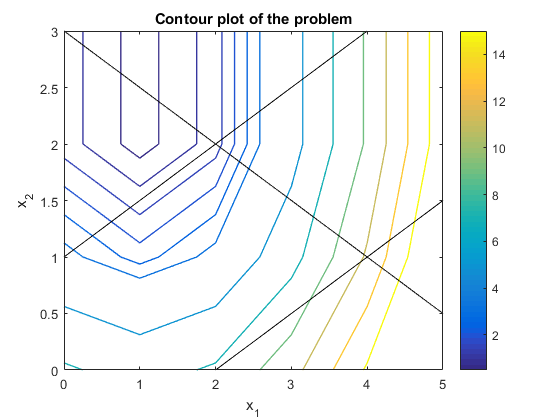
\includegraphics{exe3_contour_plot.png}
	\caption{A contour plot of the problem.}
	\label{fig:exe3_contour_plot}
\end{figure}



